\documentclass{article}
\usepackage{v-problem}
\vgeometry
\usepackage{xparse}
\usepackage{expl3}

\ExplSyntaxOn
\NewDocumentCommand\tzbboxx{ O{red} r() d() }
{
  \IfNoValueTF { #3 }
  {
    \draw[#1] (0,0) rectangle (#2);
  }
  {
    \draw[#1] (#2)  rectangle (#3);
  }
}

\NewDocumentEnvironment{ twice }
	{ O{\ttfamily} +b }
    {
    \flag_new:n {fn}
	\if_int_compare:w 5 > 7 
	#1#2
	\flag_raise:n {fn}
	\flag_show:n {fn}
	\else:
	#2
	\flag_show:n {fn}
	\fi:    
    } {}
    
    
\NewDocumentEnvironment{assemble}
{ O{P} +b }
{
\str_const:Nn \l_my_str {S}
\str_const:Nn \l_myy_str {#1}
\str_if_eq:NNTF \l_my_str \l_myy_str

	{
		\begin{tikzpicture}
		\def\C{GREENA}
		#2
		\end{tikzpicture}		
	} 
	{
		\begin{tikzpicture}
		\def\C{PINKA}
		#2
		\end{tikzpicture}	
	}
} {}
\ExplSyntaxOff


\begin{document}
\vtitle[KINEMATICS]

\def\pn{06}
\def\book{Irodov}
\def\page{14}
\def\gdrive{https://drive.google.com/drive/folders/1aHjhjudPOdhQn8gGal6h63lSRcbbpzoW?usp=share_link}

\def\question{
Two particles, $1$ and $2$, move with constant velocities $v_1$ and $v_2$ along two mutually perpendicular straight lines toward the intersection point $O$. At the moment $t = 0$ the particles were located at the distances $l_1$ and $l_2$ from the point $O$. How soon will the distance between the particles become the smallest? What is it equal to?
}

\def\option{
}


\vspace*{\fill}
\begin{tikzpicture}
	\node[qnumber] (n) at (0, 0)[scale=2] {$\pn.$};
	\node[question] (q) [right=2mm of n.east] {\question};
	\tzline[divider]<-0.125, 0> (q.north west)(q.south west);
	\node[format] (f) at  (q.south east){[\book \quad \page]};
	%\node[diagram] (d) [below=2cm of q.south] {\diagram};
	%\node[option] (o) [below=1cm of d.south] {\option};
\end{tikzpicture}	
\vspace*{\fill}
\begin{center}
\begin{tikzpicture}
	\tzcoor*(0, 0)(O){$O$}[br]
	
	\tzline+[->, thick]($(O)+(-4, 0)$)(1, 0){$v_1$}[ar]
	\tzline+[dashed](O)(-4, 0)
	\tzdot*($(O)+(-4, 0)$)(5pt)
	\tzline[|<->|]<0, -0.5>(O)($(O)+(-4, 0)$){$l_1$}[midway, below]

	\tzline+[->, thick]($(O)+(0, 4)$)(0, -1){$v_2$}[l]
	\tzline+[dashed](O)(0, 4)
	\tzdot*($(O)+(0, 4)$)(5pt)
	\tzline[|<->|]<0.5, 0>(O)($(O)+(0, 4)$){$l_2$}[midway, right]
\end{tikzpicture}
\end{center}
\vspace*{\fill}

\pagebreak

\begin{center}
\begin{tikzpicture}
	\tzcoor*(0, 0)(O){$O$}[br]
	\tzcoor*($(O)+(-4, 0)$)(A){$A$}[bl]
	\tzcoor*($(O)+(0, 4)$)(B){$B$}[al]
	\tzcoor*($(A)!0.35!(O)$)(V1)(5pt)
	\tzcoor*($(B)!0.35!(O)$)(V2)(5pt)
	
	\tzline+[->, thick](V1)(1, 0){$v_1$}[ar]
	\tzline+[->, thick](V2)(0, -1){$v_2$}[l]
	
	\tzline[dashed](O)(A)
	\tzline[dashed](O)(B)
	\tzline[|<->|]<0, -0.5>(O)(A){$l_1$}[midway, below]
	\tzline[|<->|]<0.5, 0>(O)(B){$l_2$}[midway, right]
	
	\tzline[|<->|]<0, -1>(A)(V1){$v_1t$}[midway, below]
	\tzline[|<->|]<1, 0>(B)(V2){$v_2t$}[midway, right]
	
	\tzline[|<->|]<0, -1>(V1)(O){$l_1-v_1t$}[midway, below]
	\tzline[|<->|]<1, 0>(V2)(O){$l_2-v_2t$}[midway, right]

	\tzline[dashed](V1)(V2){$s$}[sloped, midway, above]
\end{tikzpicture}
\end{center}

\addtolength{\jot}{3ex}
\begin{align}
s = \sqrt{\left(l_1-v_1t\right)^2 + \left(l_2-v_2t\right)^2} 
\end{align}
For $s$ to be minimum\_ 
\begin{align*}
\dfrac{\d{s}}{\d{t}} = 0
\end{align*}

\pagebreak
\begin{align*}
\dfrac{\d{s}}{\d{t}} &= \dfrac{1}{2\sqrt{\left(l_1-v_1t\right)^2 + \left(l_2-v_2t\right)^2}} \times \left(2\left(l_1-v_1t\right)\left(-v_1\right) + 2\left(l_2-v_2t\right)\left(-v_2\right) \right)  \\
\end{align*}

\begin{align*}
\dfrac{\d{s}}{\d{t}} &= 0 \\
\left(2\left(l_1-v_1t\right)\left(-v_1\right) + 2\left(l_2-v_2t\right)\left(-v_2\right) \right) &= 0 \\
-v_1l_1 + v_1^2t - v_2l_2 + v_2^2t &= 0\\
\left(v_1^2+v_2^2\right)t &= v_1l_1 + v_2l_2\\
\Aboxed{t &= \dfrac{v_1l_1 + v_2l_2}{\left(v_1^2+v_2^2\right)}} \ans
\end{align*}

\pagebreak
Now put the value of $t$ in equation (1)
\begin{align*}
s_{\textit{min}} &= \sqrt{\left(l_1-v_1t\right)^2 + \left(l_2-v_2t\right)^2} \bigg\rvert_{t=\dfrac{v_1l_1 + v_2l_2}{\left(v_1^2+v_2^2\right)}}\\
 &= \sqrt{\left( l_1 -v_1 \left( \dfrac{v_1l_1 + v_2l_2}{\left(v_1^2+v_2^2\right)} \right) \right)^2 + \left( l_2 -v_2 \left( \dfrac{v_1l_1 + v_2l_2}{\left(v_1^2+v_2^2\right)} \right) \right)^2 }\\
 &= \sqrt{\left( \dfrac{ l_1v_1^2 + l_1v_2^2 -v_1^2l_1 -v_1 v_2l_2}{\left(v_1^2+v_2^2\right)} \right)^2 + \left( \dfrac{ l_2v_1^2 + l_2v_2^2 -v_2v_1l_1 - v_2^2l_2}{\left(v_1^2+v_2^2\right)} \right)^2 }\\
 &= \dfrac{1}{\left( v_1^2 + v_2^2\right)}\sqrt{\textcolor{PINKD}{l_1^2v_2^4} + \textcolor{ORANGED}{v_1^2v_2^2l_2^2} - 2v_1v_2^3l_1l_2 + \textcolor{ORANGED}{l_2^2v_1^4} + \textcolor{PINKD}{v_1^2v_2^2l_1^2} - 2v_1^3v_2l_1l_2}\\
 &= \dfrac{1}{\left( v_1^2 + v_2^2\right)} \sqrt{\left(v_1^2+v_2^2\right)\left[ l_1^2v_2^2 + l_2^2v_1^2-2v_1v_2l_1l_2\right]}\\
 &= \dfrac{\left| l_1v_2-l_2v_1 \right|}{\sqrt{v_1^2+v_2^2}} \ans
\end{align*}
\pagebreak

\vspace*{\fill}
\begin{center}
	\fbox{\qrcode[height=2cm]{\gdrive}}
\end{center}
\vspace*{\fill}

\pagebreak

\begin{center}
\NewDocumentCommand {\margins} { O{#3} m O{#1} m } {(#1,#2,#3,#4)}
%\margins{a}{b}

\begin{twice}
    Hello world!
\end{twice}

\begin{tikzpicture}
\tzbboxx[GREEND](1, 0)(5, 1)
\tzcoor(3,  4)(A)
\tzgetxyval(A){\x}{\y}
\tzdot*(\x, \y)

\end{tikzpicture}

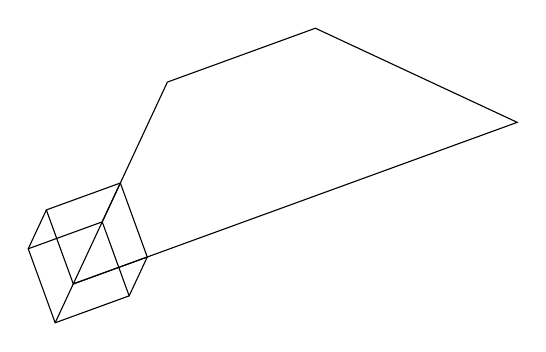
\begin{tikzpicture}[rotate=20]
\draw (0,0,0) -- (0,1,0) -- (1,1,0) -- (1,0,0) -- cycle;
\draw (0,0,1) -- (0,1,1) -- (1,1,1) -- (1,0,1) -- cycle;
\draw (0,0,0) -- (0,0,1);
\draw (1,0,0) -- (1,0,1);
\draw (0,1,0) -- (0,1,1);
\draw (1,1,0) -- (1,1,1);
\draw (0,0) -- (2,2) -- (4,2) -- (6,0) -- cycle;
\end{tikzpicture}
\end{center}

\begin{assemble}[P]
	\node[qnumber, \C] (n) at (0, 0)[scale=2] {$\pn.$};
	\node[question] (q) [right=2mm of n.east] {\question};
	\tzline[divider, \C]<-0.125, 0> (q.north west)(q.south west);
	\node[format] (f) at  (q.south east){[\book \quad \page]};
\end{assemble}

\end{document}
